\documentclass[../../../../main.tex]{subfiles}
\begin{document}
\section{User Interaction}
All of these features require me to know about how mouse events are handled in JavaFX since all of these actions require some kind of mouse input. I used these websites\cite{eventsJava} to get a deeper understanding of how they worked. Events are essentially objects with attributes that describe the event that just occurred. For example an attribute could tell you the position of the event. They are quite simple to use and if required I will give specifics when needed.

\subsection{Coordinates}
I used the algorithm I designed in the design section and implemented it as a method in the input layer class. I then bound this method to the \texttt{OnMouseMoved} mouse event in the input layer constructor, so the coordinates would update whenever the moused moved in the plot pane. So I added this to the input layer constructor:
\begin{minted}[
frame=lines,
framesep=2mm,
breaklines
]{java}
this.canvas.setOnMouseMoved(event -> drawCoords(event));
\end{minted}
Here is the \texttt{drawCoords()} method:
\begin{minted}[
frame=lines,
framesep=2mm,
linenos,
breaklines
]{java}
// draw the coordinates
private void drawCoords(MouseEvent event) {
	// clear the previous coordinates
	clearCanvas();
	// get the coordinates
	double x = (event.getX() * this.pixelWorthX.doubleValue()) + this.minX.doubleValue();
	double y = this.maxY.doubleValue() - (event.getY() * this.pixelWorthY.doubleValue());
	// round the coordinates to 2 decimal places
	String sX = new DecimalFormat("#.##").format(x);
	String sY = new DecimalFormat("#.##").format(y);
	String out = "(" + sX + "," + sY + ")";
	// draw the coordinates to the canvas
	gc.setLineWidth(1);
	gc.strokeText(out, 0, 10);
}
\end{minted}
It works perfectly and an image of what it looks like is shown below. I asked Palvinder, the stakeholder who suggested this feature, about what he thought of the implementation and he said that it was \textit{``exactly how I envisioned it to be''}.
\begin{figure}[H]
	\centering
	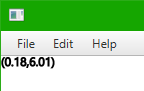
\includegraphics[width=0.4\textwidth]{images/coords}
	\caption{Coordinates in Action}
\end{figure}
\newpage
\subsection{Pan}
The panning feature was quite hard to implement due to the lack of clear documentation on \texttt{DragEvent}. From lots of searching I found out that I had to call \texttt{startFullDrag()} method when the drag is initiated. Using this information I added these lines to the input layer constructor:
\begin{minted}[
frame=lines,
framesep=2mm,
breaklines
]{java}
this.canvas.setOnMousePressed(event -> dragEntered(event));
this.canvas.setOnMouseDragged(event -> pan(event));
\end{minted}
I also added 4 new attributes of type double to the input layer class, \texttt{previousX}, \texttt{previousY}, \texttt{currentX} and \texttt{currentY}. Here are the two methods used in the previous snippet of code \texttt{dragEntered()} and \texttt{pan()}:
\begin{minted}[
frame=lines,
framesep=2mm,
linenos,
breaklines
]{java}
// when drag starts initiate the full-drag sequence
private void dragEntered(MouseEvent event) {
	// only initiate the drag if its the left mouse button
	if (event.isPrimaryButtonDown()) {
		// start full drag
		event.setDragDetect(true);
		this.canvas.startFullDrag();
	}
}

// pan around the plotpane
private void pan(MouseEvent event) {
	if (event.isPrimaryButtonDown()) {
		// get the current mouse coordinates
		currentX = event.getX();
		currentY = event.getY();
		// get the vector of the mouse movement
		double xTrans = (previousX - currentX);
		double yTrans = (previousY - currentY);
		// update the previous values to be the current ones
		previousX = currentX;
		previousY = currentY;
		// translate the viewport
		this.maxX.set((this.pixelWorthX.doubleValue() * xTrans) + this.maxX.doubleValue());
		this.minX.set((this.pixelWorthX.doubleValue() * xTrans) + this.minX.doubleValue());
		this.maxY.set(-(this.pixelWorthY.doubleValue() * yTrans) + this.maxY.doubleValue());
		this.minY.set(-(this.pixelWorthY.doubleValue() * yTrans) + this.minY.doubleValue());
		this.changeViewport.set(!this.changeViewport.get());
	}
}
\end{minted}
\newpage
Then I tested the pan functionality. When I first held down the left mouse click button, the viewport jumped to another location and then the pan functionality worked fine, as in I could move it about. This told me that there was a problem while initiating the drag sequence. So I used breakpoints, debugging tools and the variable stack viewer in Eclipse to debug the problem:
\begin{figure}[H]
	\centering
	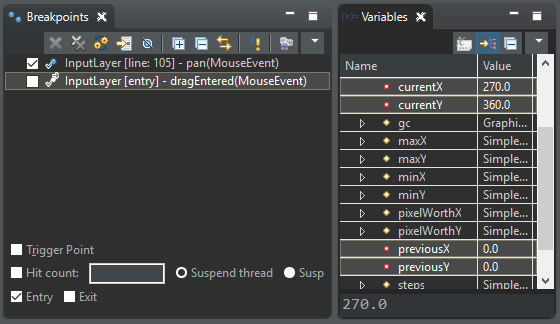
\includegraphics[width=0.6\textwidth]{images/debug}
	\caption{Coordinates in Action}
\end{figure}
From this I realized that the values for \texttt{previousX} and \texttt{previousY} were the last values in the previous drag which caused the viewport to jump when initiating the drag. To fix this when entering the drag I gave them the value of the current location of the cursor:
\begin{minted}[
frame=lines,
framesep=2mm,
linenos,
breaklines
]{java}
// when drag starts initiate the full-drag sequence
private void dragEntered(MouseEvent event) {
	// only initiate the drag if its the left mouse button
	if (event.isPrimaryButtonDown()) {
		// need to initialize the values of previousX and previousY
		previousX = event.getX();
		previousY = event.getY();
		// start full drag
		event.setDragDetect(true);
		this.canvas.startFullDrag();
	}
}
\end{minted}
This fixed the issue, although an exception seems to be thrown every time the drag is initiated:
\begin{minted}[
frame=lines,
framesep=2mm,
breaklines
]{console}
Exception in thread "JavaFX Application Thread" java.lang.IllegalStateException:
Cannot start full drag outside of DRAG_DETECTED event handler
\end{minted}
However the panning feature works so this exception can be ignored. Evidence of it working will be shown in the testing section in video form.
\newpage
\subsection{Zoom}
I used the algorithm I designed in the design section and implemented it as a method in the input layer class, with some slight changes talked about in the next paragraph. I then bound this method to the \texttt{OnScroll} scroll event in the input layer constructor, so that the it would zoom in or out when scrolling. This is what the input layer constructor is and this is the final change:
\begin{minted}[
frame=lines,
framesep=2mm,
linenos,
breaklines
]{java}
public InputLayer() {
	// call the super constructor
	super();
	// update pixel worth when the canvas changes size
	this.canvas.heightProperty().addListener(event -> updatePixelWorth());
	this.canvas.widthProperty().addListener(event -> updatePixelWorth());
	// bind the mouse events to their respective actions
	this.canvas.setOnMousePressed(event -> dragEntered(event));
	this.canvas.setOnMouseDragged(event -> pan(event));
	this.canvas.setOnScroll(event -> zoom(event));
	this.canvas.setOnMouseMoved(event -> drawCoords(event));
}
\end{minted}
When the scroll event is triggered it is an object with various attributes. One of them is the \textit{deltaY} attribute. It is an integer and it tells us if the scroll wheel is being scrolled down or up. If it is positive it is being scrolled down and if it is negative it is being scrolled up. So using this knowledge I took my algorithm I designed and adapted it to to implemented \texttt{zoom()} method:
\begin{minted}[
frame=lines,
framesep=2mm,
linenos,
breaklines
]{java}
// zoom in and out
private void zoom(ScrollEvent event) {
	double zoomFactor = 1.05;
	// this is whether it is scrolling up or down
	double deltaY = event.getDeltaY();
	// get the coordinates
	double x = (event.getX() * this.pixelWorthX.doubleValue()) + this.minX.doubleValue();
	double y = this.maxY.doubleValue() - (event.getY() * this.pixelWorthY.doubleValue());
	// if scrolling down shrink the viewport instead
	if (deltaY > 0) {
		zoomFactor = 1 / zoomFactor;
	}
	// translate the viewport to the origin, scale the viewport,
	// translate the viewport back and set the new values for the viewport
	this.minX.set((this.minX.doubleValue() - x) * zoomFactor + x);
	this.maxX.set((this.maxX.doubleValue() - x) * zoomFactor + x);
	this.minY.set((this.minY.doubleValue() - y) * zoomFactor + y);
	this.maxY.set((this.maxY.doubleValue() - y) * zoomFactor + y);
	// update and notify the plotpane
	this.updatePixelWorth();
	this.changeViewport.set(!this.changeViewport.get());
}
\end{minted}
It works perfectly and evidence of it in action will be shown in video form in the testing section. Using alone images will not be able to capture the zooming in and out.
\newpage
\subsection{Save Picture}
I found these two posts\cite{savePlot,snapshotJava}, which I combined to be able to save the image where the user wants and with any name. To create the context menu, the right click menu, I used this example\cite{contextMenu}. I edited and inserted this code to add a right click menu at the end of the plot pane constructor:
\begin{minted}[
frame=lines,
framesep=2mm,
linenos,
breaklines
]{java}
// create a right click menu
ContextMenu contextMenu = new ContextMenu();
MenuItem save = new MenuItem("Save as Picture");
contextMenu.getItems().addAll(save);
// set an action to call the savePlot() method when clicking the save button
save.setOnAction(new EventHandler<ActionEvent>() {
	@Override
	public void handle(ActionEvent event) {
		savePlot();
	}
});
// when right clicking open the menu
this.setOnContextMenuRequested(
		event -> contextMenu.show(this.getScene().getWindow(), event.getScreenX(), event.getScreenY()));
\end{minted}
I then created the \texttt{savePlot()} method that is called when the \textit{``Save as Picture''} menu item is clicked:
\begin{minted}[
frame=lines,
framesep=2mm,
linenos,
breaklines
]{java}
// save picture of plot
private void savePlot() {
	// create the file navigator object
	FileChooser fileChooser = new FileChooser();
	// set extension filter (make the image of format png)
	fileChooser.getExtensionFilters().add(new FileChooser.ExtensionFilter("png files (*.png)", "*.png"));
	// prompt user to select a file
	File file = fileChooser.showSaveDialog(null);
	if (file != null) {	//if the user chose to save then snapshot the pane
		try {
			// create the snapshot of the pane
			WritableImage snapshot = this.snapshot(new SnapshotParameters(), null);
			RenderedImage renderedImage = SwingFXUtils.fromFXImage(snapshot, null);
			// write the snapshot to the chosen file
			ImageIO.write(renderedImage, "png", file);
		} catch (IOException ex) {
			ex.printStackTrace();
		}
	}
}
\end{minted}
\newpage
I then tried to save an image of the plot and it worked perfectly:
\begin{figure}[H]
\centering
\begin{minipage}{.5\textwidth}
	\centering
  	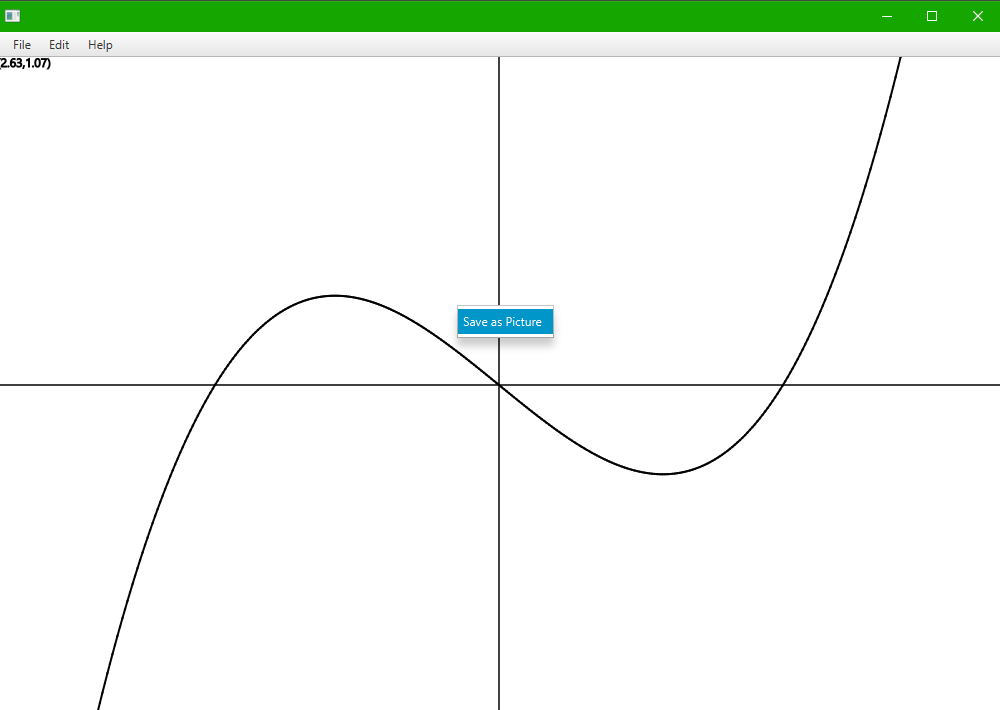
\includegraphics[width=.8\textwidth]{images/contextMenu}
	\caption{The Right Click Menu}
\end{minipage}%
\begin{minipage}{.5\textwidth}
	\centering
	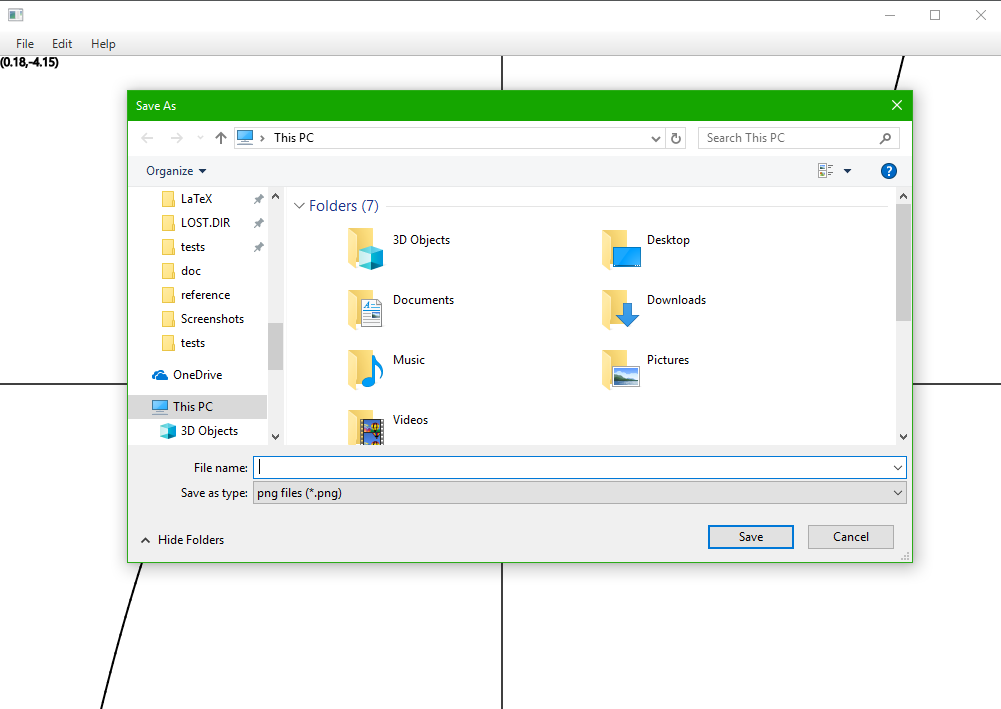
\includegraphics[width=.8\textwidth]{images/fileNavigator}
	\caption{The File Navigator to Save the File}
\end{minipage}
\end{figure}
\begin{figure}[H]
	\centering
	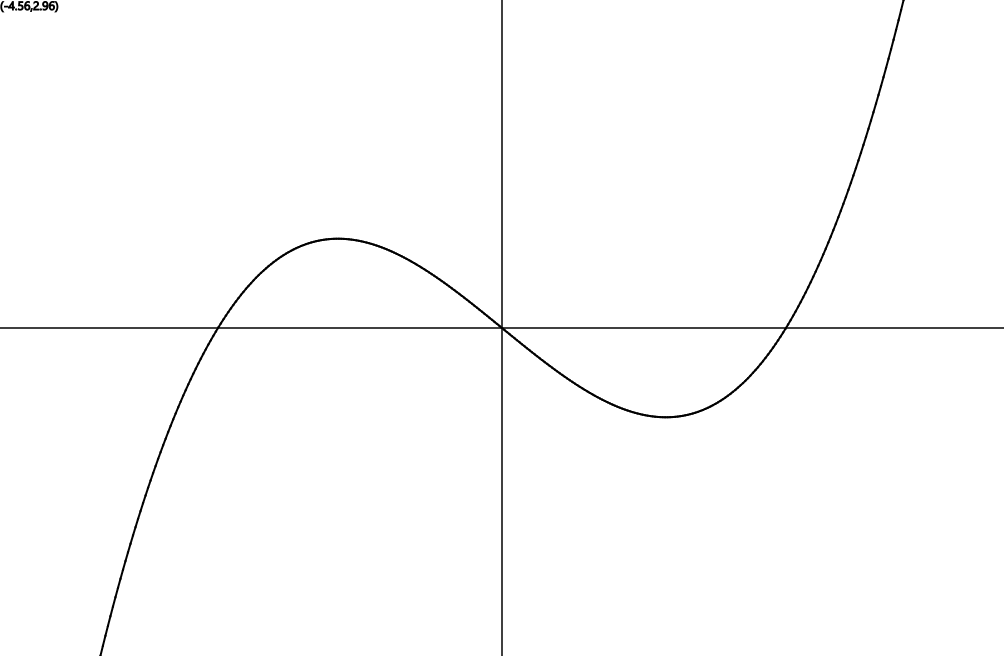
\includegraphics[width=0.8\textwidth]{images/withCoords}
	\caption{The Image Produced}
\end{figure}
A recording of the process to save will be done during the overall testing.
\newpage\noindent
I let the stakeholder who originally asked for this feature, Lewis, try it and he said that he said it was all good except for the \textit{``coordinates that were shown in the top left corner''} and he said that he didn't want it in the saved picture. I took his suggestion and tried to fix it. Since the coordinates are part of the input layer, I fixed this by removing the input layer canvas, taking the snapshot and then readding the input layer canvas. It worked, so I showed Lewis again and he said it was \textit{``great''}. Here is the code and evidence for the updated feature:
\begin{minted}[
frame=lines,
framesep=2mm,
linenos,
breaklines
]{java}
// save picture of plot
private void savePlot() {
	// create the file navigator object
	FileChooser fileChooser = new FileChooser();
	// set extension filter
	fileChooser.getExtensionFilters().add(new FileChooser.ExtensionFilter("png files (*.png)", "*.png"));
	// set extension filter (make the image of format png)
	File file = fileChooser.showSaveDialog(null);
	if (file != null) {	//if the user chose to save then snapshot the pane
		try {
			// remove input layer canvas, the top node, to not show the coords
			this.getChildren().remove(this.getChildren().size() - 1);
			// create the snapshot of the pane
			WritableImage snapshot = this.snapshot(new SnapshotParameters(), null);
			RenderedImage renderedImage = SwingFXUtils.fromFXImage(snapshot, null);
			// write the snapshot to the chosen file
			ImageIO.write(renderedImage, "png", file);
		} catch (IOException ex) {
			ex.printStackTrace();
		} finally {
			// readd the input layer
			this.getChildren().add(inputLayer.getCanvas());
		}
	}
}
\end{minted}
\begin{figure}[H]
	\centering
	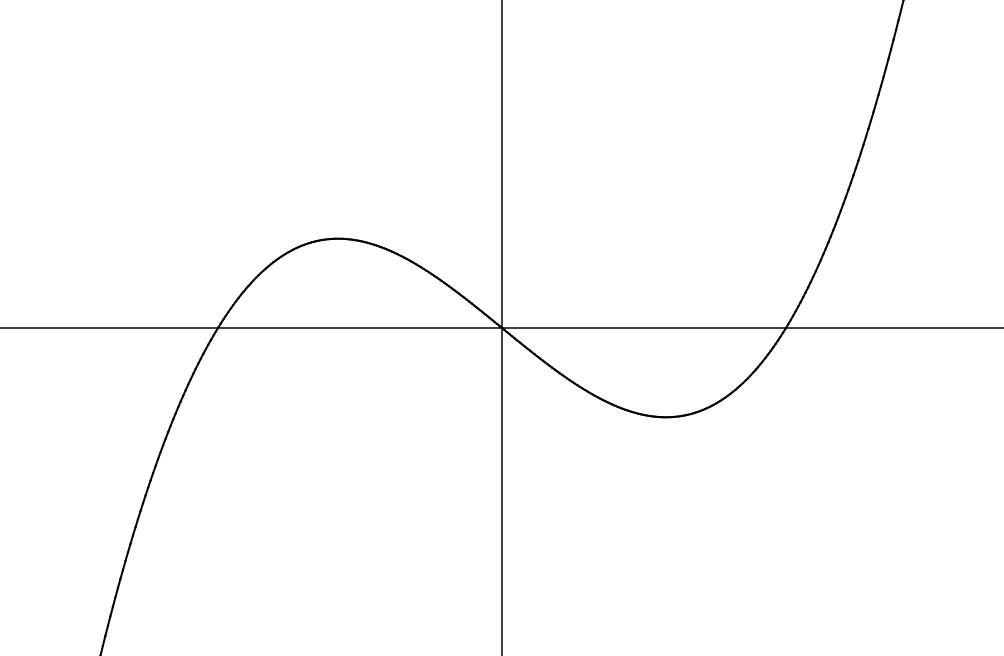
\includegraphics[width=0.45\textwidth]{images/withoutCoords}
	\caption{The Image Produced}
\end{figure}
\end{document}